Las razones por las cuales se toma la decisión de fabricar la estructura del brazo mediante impresión 3D se detallan a continuación:

\begin{itemize}
  \item Cumplir con el requisito de replicabilidad y asequibilidad: Una de las bases del proyecto es que pueda ser reproducible a bajo coste tanto de recursos como de tiempo. Se decide por tanto construir la estructura física del brazo mediante técnicas de impresión 3D ya que están altamente extendidas y son cada vez mas asequibles.
  
  \item Características físicas del material: El plástico utilizado para la impresión es ligero y suficientemente resistente para soportar las cargas para las que esta pensado el manipulador.
  
  \item Disponibilidad de impresora 3D: Dado que la universidad es capaz de proveer al equipo con una impresora 3D funcional, los costes del proyecto se abaratan si la estructura es realizada con los medios de los que la universidad ya dispone.
  
  \item Simplificar el proceso de mejora y personalización: Debido a la naturaleza OpenSoftware y OpenHardware del proyecto se espera que las personas interesadas puedan contribuir a el mejorándolo y/o personalizándolo. La impresión 3D facilita estas acciones.
\end{itemize}

La impresora que la Universidad pone a disposición del equipo de trabajo es la Ultimaker 3 Extended la cual es capaz de imprimir en una alta variedad de materiales. El equipo ha considerado los siguientes materiales:

\begin{itemize}
    \item PLA (ácido poliláctico)\cite{noauthor_acido_2020}: Este material imprime de manera segura con alta precisión dimensional y una resistencia a la tracción excepcional. Permite grandes velocidades de impresión. Es biodegradable ya que se obtienen a partir de almidón de maíz o de yuca o mandioca, o de caña de azúcar. 
    \item ABS (acrilonitrilo butadieno estireno)\cite{noauthor_acrilonitrilo_2020}: Este material presenta buena adhesión entre capas y con una resistencia a temperaturas de hasta 85ºC. Permite obtener buenos detalles estéticos.
    \item Ultimaker Nylon: Este material es un tipo de poliamida basada en PA6/66. Presenta una absorción de humedad reducida así como una capacidad considerable de resistencia ante tensiones mecánicas. También presenta un bajo coeficiente de fricción.
    \item CPE y CPE+: Este material presenta una alta estabilidad dimensional, con buena resistencia al impacto y a la temperatura. Debido a su alta solidez y su estabilidad dimensional ofrece un buen rendimiento mecánico y gran resistencia al desgaste.
\end{itemize}

Debido a la naturaleza del proyecto el equipo ha decidido emplear materiales con alta resistencia mecánica y el Ultimaker Nylon junto con el CPE cumplen con dicha característica.

Aprovechando la licencia GPL 3.0 se ha recuperado el modelo 3D proporcionado por UFactory como punto de partida. A partir de este modelo se han impreso las piezas que hemos decidido conservar para nuestro proyecto.

\begin{figure}[H]
    \centering
    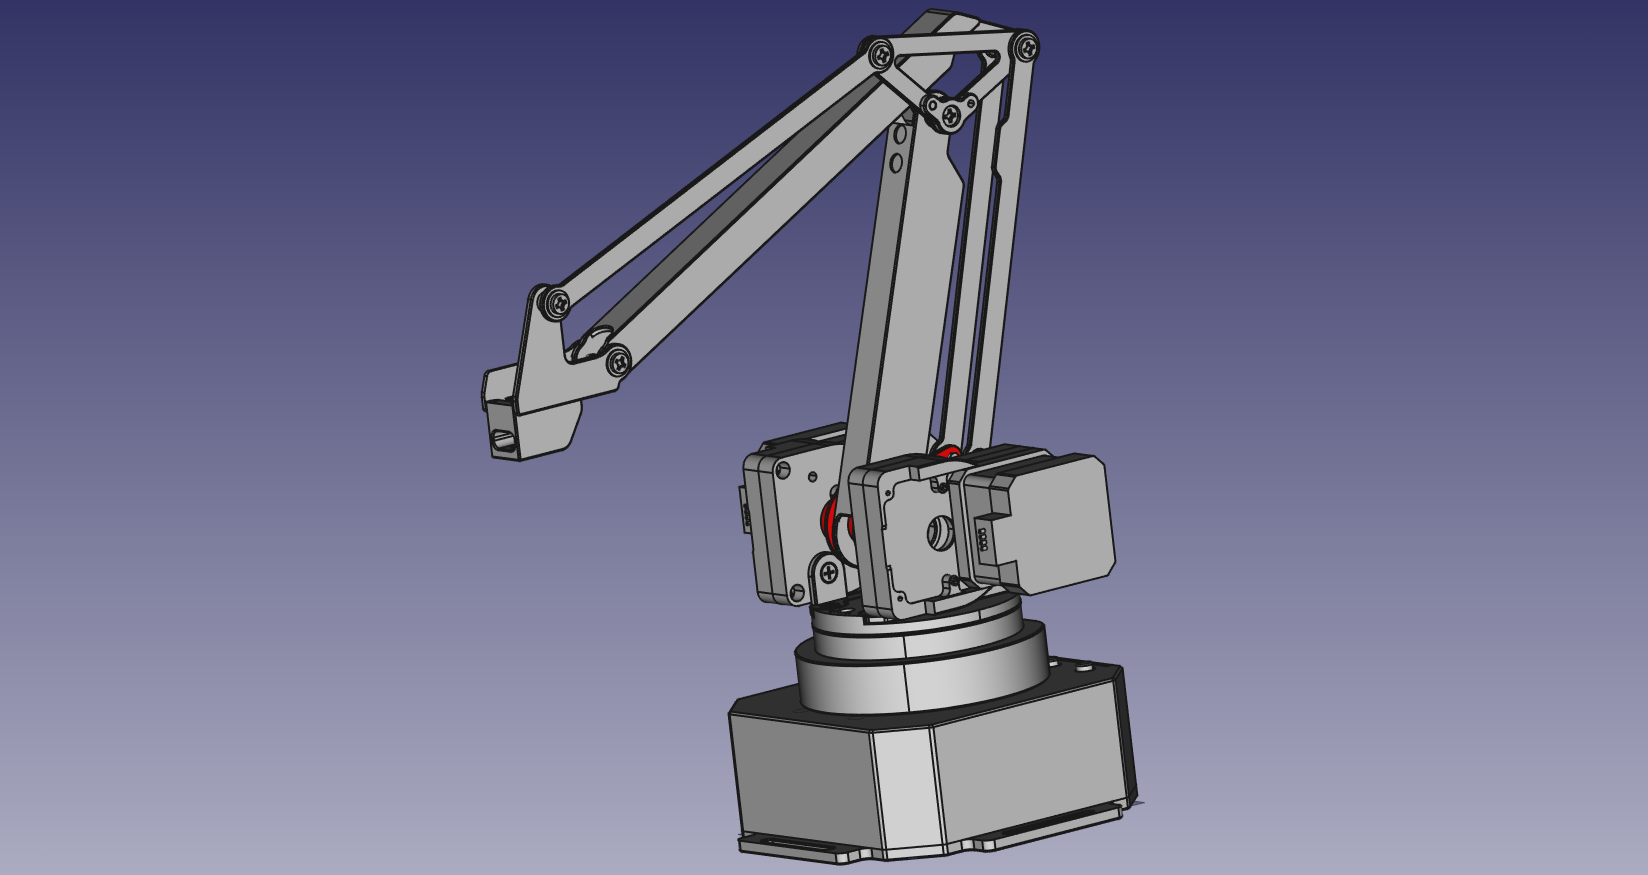
\includegraphics[width=12cm]{pictures/brazo_vista_3d_inicial.png}
    \caption{Concepto inicial del brazo robótico}
    \label{fig:manipulador_inicial}
\end{figure}

Las herramientas que han sido empleadas para visualizar y modificar el modelo y posteriormente imprimir las piezas han sido respectivamente FreeCAD y Slic3r.

\begin{figure}[H]
    \centering
    
\includegraphics[width=6cm]{pictures/freeCAD.jpg}
    
\includegraphics[width=6cm]{pictures/slic3r_logo.jpg}
    \caption{Herramientas utilizadas}
    \label{fig:herramientas_3d}
\end{figure}

El flujo de trabajo que se ha seguido desde el modelo 3D hasta la impresión de una pieza ha sido el siguiente.

\begin{figure}[H]
    \centering
    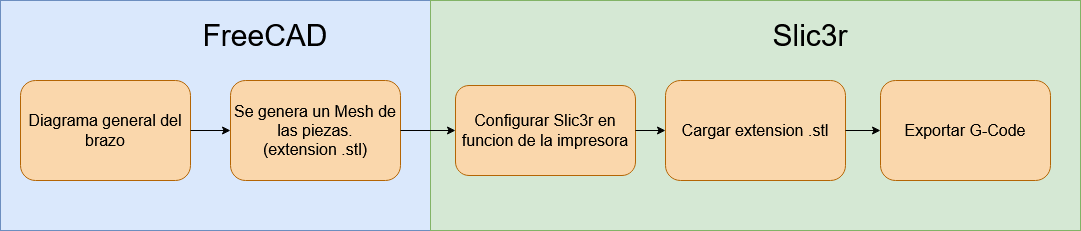
\includegraphics[width=.9\linewidth]{pictures/flujo_trabajo_impresion.png}
    \caption{Flujo de trabajo de la impresión 3D}
    \label{fig:flujo_3d}
\end{figure}

La estructura del brazo es pantográfica. Un pantógrafo es un sistema de enlaces mecánicos que reproduce el movimiento de un punto de los enlaces en un segundo punto, normalmente a un tamaño mas pequeño o mas grande. Se origino en el siglo XVII y su aplicación mas conocida es como instrumento de dibujo. 

\begin{figure}[H]
    \centering
    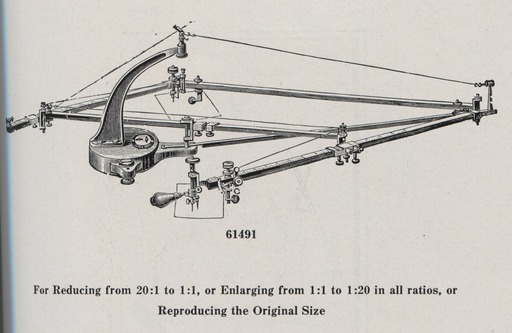
\includegraphics[width=.9\linewidth]{pictures/link-to-elliott-p149-suspended-pantograph-sf0.jpg}
    \caption{Una estructura pantográfica}
    \label{fig:flujo_3d}
\end{figure}

El hecho de que que la estructura del brazo sea pantógrafo permite controlar todas las articulaciones mediante motores ubicados en la base. Esto es de especial importancia ya que hace posible que las articulaciones finales no carguen con el peso de los motores permitiendo emplear materiales como el plástico para la construcción de la estructura y además dando capacidad al brazo para levantar cargas mas pesadas.




